\documentclass{beamer}

% choose theme (warning, to use the UniBern theme you need to copy the files beamerthemeUniBern.sty and ublogo.pdf in the same directory)
\usetheme{UniBern}

% packages

\usepackage{graphicx}
\usepackage{hyperref} % allows clickable urls
\usepackage{tikz}

\newcommand\blfootnote[1]{%
	\begingroup
	\renewcommand\thefootnote{}\footnote{#1}%
	\addtocounter{footnote}{-1}%
	\endgroup
}

% define title page
\title{Bayesian workflow for disease transmission modeling in Stan}
\subtitle{{\small Eustat -- XXXIII Seminario Internacional de Estadistica} }
\author{Julien Riou, MD PhD}
\date{Institute of Social and Preventive Medicine, University of Bern, Switzerland}
\institute{institute}

% begin document
\begin{document}
	
\frame{\titlepage}

\frame{
	\frametitle{Preface}
	\begin{itemize}
		\item Objective: fit transmission models in Stan 
		\item Based on Grinsztajn et al., 2020
		\item Prerequisites:
			\begin{itemize}
				\item Bayesian inference
				\item Programming with R
				\item Basic programming with Stan
			\end{itemize}
		\item All material is available on 
	\end{itemize}
}

\frame{
	\frametitle{Outline}
	\begin{itemize}
		\item Introduction
		\item (Quick notice: Bayesian inference)
		\item (Quick notice: programming with Stan)
		\item Simple SIR
		\item Using simulated data
		\item Scaling up ODE-based models
		\item Extensions 
	\end{itemize}
	
	\vspace{4em}
	\blfootnote{Ref: Grinsztajn et al.~(2020)}
}

\frame{
	\frametitle{Introduction}
	Models of disease transmission:
	\begin{itemize}
		\item Interpretability: mechanistic, phenomenological
		\pause
		\item Data-generating mechanisms: incubation, contagion, immunity...
		\pause
		\item Scale: agent-based, population-based
		\pause
		\item Framework: deterministic, stochastic
	\end{itemize}
	\pause
	
	\vspace{2em}
	Mechanistic + population-based + deterministic 
	
	\vspace{1em}\hspace{2em} $\rightarrow$ \alert{ODE-based compartmental model} (e.g., SIR)
}

\frame{
	\frametitle{Introduction}
	ODE-based compartmental model:
	\begin{itemize}
		\item Divide the population into homogeneous groups (compartments)
		\pause
		\item Define flows between compartments with differential equations
		\pause
		\item Define initial conditions
		\pause
		\item Solve for the time-dependent volume in each compartment
	\end{itemize}
	\vspace{1em}
	\pause
	
	\begin{figure}
		\centering
		\scalebox{.8}{
		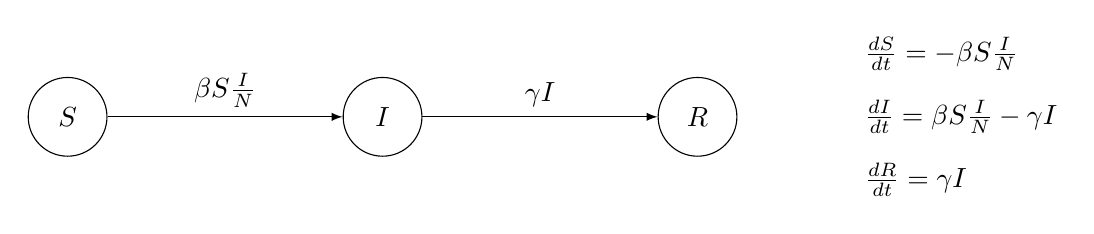
\begin{tikzpicture}
			\node[circle, draw, inner sep=0pt, minimum size=1cm] (S) at (0,0) {$S$};
			\node[circle, draw, inner sep=0pt, minimum size=1cm] (I) at (4,0) {$I$};
			\node[circle, draw, inner sep=0pt, minimum size=1cm] (R) at (8,0) {$R$};
			
			\draw[->,>=latex] (S) edge node[above] { $\beta S \frac{I}{N}$} (I);
			\draw[->,>=latex] (I) edge node[above] { $\gamma I$} (R);
			
			\node[anchor=west] at (10,.8) {$	\frac{dS}{dt} = - \beta S \frac{I}{N}$};
			\node[anchor=west] at (10,0) {$	\frac{dI}{dt} = \beta S \frac{I}{N} - \gamma I $};
			\node[anchor=west] at (10,-.8) {$\frac{dR}{dt} = \gamma I $};
		\end{tikzpicture}
	}
	\end{figure}
}


\frame{
	\frametitle{Introduction}
	
	Simulate in \texttt{R} with package \texttt{deSolve}:
	
	\begin{itemize}
		\item set compartments and differential equations
	\end{itemize}
	\begin{figure}
		\centering
		\includegraphics[width=0.55\linewidth]{figures/simsir3.png}
	\end{figure}
	\pause
	\begin{itemize}
		\item set (fixed) values for $\beta$, $\gamma$, $N(0)$ and $I(0)$
	\end{itemize}
	\begin{figure}
		\centering
		\includegraphics[width=0.45\linewidth]{figures/simsir1.png}
		\includegraphics[width=0.45\linewidth]{figures/simsir2.png}
	\end{figure}
}


\frame{
	\frametitle{Introduction}
	
	Simulate in \texttt{R} with package \texttt{deSolve}:
	
	\begin{itemize}
		\item solve ODE system numerically (Runge-Kutta 4th order)
	\end{itemize}
	\begin{figure}
		\centering
		\includegraphics[width=0.7\linewidth]{figures/simsir4.png}
	\end{figure}
}

\frame{
	\frametitle{Introduction}
	
	Simulate in \texttt{R} with package \texttt{deSolve}:
	
	\begin{figure}
		\centering
		\includegraphics[width=0.7\linewidth]{figures/example_sir1.pdf}
	\end{figure}
}
















\frame{
	\frametitle{Acknowledgements \& ressources}
	\begin{itemize}
		\item Michael Bettencourt's \textit{Introduction to Stan} \url{https://betanalpha.github.io/assets/case_studies/stan_intro.html}
		\item Daniel Lee's \textit{ODEs in Stan} \\ \url{https://youtu.be/hJ34_xJhYeY}
		\item Richard McElreath's \textit{Statistical rethinking} \url{https://youtu.be/4WVelCswXo4}
	
	\end{itemize}
	
}

\end{document}
